\documentclass{article}
\usepackage[utf8]{inputenc}
\usepackage[spanish]{babel}
\usepackage{listings}
\usepackage{graphicx}
\graphicspath{ {images/} }
\usepackage{cite}
\usepackage{amssymb, amsmath}
\usepackage{geometry}
\geometry{
textheight=23cm
}

%arduino
 %%%%%%%%%%%%%%%%%%%%%%%%%%%%%%%%%%%%%%%%%%%%%%%%%%%%%%%%%%%%%%%%%%%%%%%%%%%%%%%% 
%%% ~ Arduino Language - Arduino IDE Colors ~                                  %%%
%%%                                                                            %%%
%%% Kyle Rocha-Brownell | 10/2/2017 | No Licence                               %%%
%%% -------------------------------------------------------------------------- %%%
%%%                                                                            %%%
%%% Place this file in your working directory (next to the latex file you're   %%%
%%% working on).  To add it to your project, place:                            %%%
%%%     %%%%%%%%%%%%%%%%%%%%%%%%%%%%%%%%%%%%%%%%%%%%%%%%%%%%%%%%%%%%%%%%%%%%%%%%%%%%%%%% 
%%% ~ Arduino Language - Arduino IDE Colors ~                                  %%%
%%%                                                                            %%%
%%% Kyle Rocha-Brownell | 10/2/2017 | No Licence                               %%%
%%% -------------------------------------------------------------------------- %%%
%%%                                                                            %%%
%%% Place this file in your working directory (next to the latex file you're   %%%
%%% working on).  To add it to your project, place:                            %%%
%%%     %%%%%%%%%%%%%%%%%%%%%%%%%%%%%%%%%%%%%%%%%%%%%%%%%%%%%%%%%%%%%%%%%%%%%%%%%%%%%%%% 
%%% ~ Arduino Language - Arduino IDE Colors ~                                  %%%
%%%                                                                            %%%
%%% Kyle Rocha-Brownell | 10/2/2017 | No Licence                               %%%
%%% -------------------------------------------------------------------------- %%%
%%%                                                                            %%%
%%% Place this file in your working directory (next to the latex file you're   %%%
%%% working on).  To add it to your project, place:                            %%%
%%%    \input{arduinoLanguage.tex}                                             %%%
%%% somewhere before \begin{document} in your latex file.                      %%%
%%%                                                                            %%%
%%% In your document, place your arduino code between:                         %%%
%%%   \begin{lstlisting}[language=Arduino]                                     %%%
%%% and:                                                                       %%%
%%%   \end{lstlisting}                                                         %%%
%%%                                                                            %%%
%%% Or create your own style to add non-built-in functions and variables.      %%%
%%%                                                                            %%%
 %%%%%%%%%%%%%%%%%%%%%%%%%%%%%%%%%%%%%%%%%%%%%%%%%%%%%%%%%%%%%%%%%%%%%%%%%%%%%%%% 

\usepackage{color}
\usepackage{listings}    
\usepackage{courier}

%%% Define Custom IDE Colors %%%
\definecolor{arduinoGreen}    {rgb} {0.17, 0.43, 0.01}
\definecolor{arduinoGrey}     {rgb} {0.47, 0.47, 0.33}
\definecolor{arduinoOrange}   {rgb} {0.8 , 0.4 , 0   }
\definecolor{arduinoBlue}     {rgb} {0.01, 0.61, 0.98}
\definecolor{arduinoDarkBlue} {rgb} {0.0 , 0.2 , 0.5 }

%%% Define Arduino Language %%%
\lstdefinelanguage{Arduino}{
  language=C++, % begin with default C++ settings 
%
%
  %%% Keyword Color Group 1 %%%  (called KEYWORD3 by arduino)
  keywordstyle=\color{arduinoGreen},   
  deletekeywords={  % remove all arduino keywords that might be in c++
                break, case, override, final, continue, default, do, else, for, 
                if, return, goto, switch, throw, try, while, setup, loop, export, 
                not, or, and, xor, include, define, elif, else, error, if, ifdef, 
                ifndef, pragma, warning,
                HIGH, LOW, INPUT, INPUT_PULLUP, OUTPUT, DEC, BIN, HEX, OCT, PI, 
                HALF_PI, TWO_PI, LSBFIRST, MSBFIRST, CHANGE, FALLING, RISING, 
                DEFAULT, EXTERNAL, INTERNAL, INTERNAL1V1, INTERNAL2V56, LED_BUILTIN, 
                LED_BUILTIN_RX, LED_BUILTIN_TX, DIGITAL_MESSAGE, FIRMATA_STRING, 
                ANALOG_MESSAGE, REPORT_DIGITAL, REPORT_ANALOG, SET_PIN_MODE, 
                SYSTEM_RESET, SYSEX_START, auto, int8_t, int16_t, int32_t, int64_t, 
                uint8_t, uint16_t, uint32_t, uint64_t, char16_t, char32_t, operator, 
                enum, delete, bool, boolean, byte, char, const, false, float, double, 
                null, NULL, int, long, new, private, protected, public, short, 
                signed, static, volatile, String, void, true, unsigned, word, array, 
                sizeof, dynamic_cast, typedef, const_cast, struct, static_cast, union, 
                friend, extern, class, reinterpret_cast, register, explicit, inline, 
                _Bool, complex, _Complex, _Imaginary, atomic_bool, atomic_char, 
                atomic_schar, atomic_uchar, atomic_short, atomic_ushort, atomic_int, 
                atomic_uint, atomic_long, atomic_ulong, atomic_llong, atomic_ullong, 
                virtual, PROGMEM,
                Serial, Serial1, Serial2, Serial3, SerialUSB, Keyboard, Mouse,
                abs, acos, asin, atan, atan2, ceil, constrain, cos, degrees, exp, 
                floor, log, map, max, min, radians, random, randomSeed, round, sin, 
                sq, sqrt, tan, pow, bitRead, bitWrite, bitSet, bitClear, bit, 
                highByte, lowByte, analogReference, analogRead, 
                analogReadResolution, analogWrite, analogWriteResolution, 
                attachInterrupt, detachInterrupt, digitalPinToInterrupt, delay, 
                delayMicroseconds, digitalWrite, digitalRead, interrupts, millis, 
                micros, noInterrupts, noTone, pinMode, pulseIn, pulseInLong, shiftIn, 
                shiftOut, tone, yield, Stream, begin, end, peek, read, print, 
                println, available, availableForWrite, flush, setTimeout, find, 
                findUntil, parseInt, parseFloat, readBytes, readBytesUntil, readString, 
                readStringUntil, trim, toUpperCase, toLowerCase, charAt, compareTo, 
                concat, endsWith, startsWith, equals, equalsIgnoreCase, getBytes, 
                indexOf, lastIndexOf, length, replace, setCharAt, substring, 
                toCharArray, toInt, press, release, releaseAll, accept, click, move, 
                isPressed, isAlphaNumeric, isAlpha, isAscii, isWhitespace, isControl, 
                isDigit, isGraph, isLowerCase, isPrintable, isPunct, isSpace, 
                isUpperCase, isHexadecimalDigit, 
                }, 
  morekeywords={   % add arduino structures to group 1
                break, case, override, final, continue, default, do, else, for, 
                if, return, goto, switch, throw, try, while, setup, loop, export, 
                not, or, and, xor, include, define, elif, else, error, if, ifdef, 
                ifndef, pragma, warning,
                }, 
% 
%
  %%% Keyword Color Group 2 %%%  (called LITERAL1 by arduino)
  keywordstyle=[2]\color{arduinoBlue},   
  keywords=[2]{   % add variables and dataTypes as 2nd group  
                HIGH, LOW, INPUT, INPUT_PULLUP, OUTPUT, DEC, BIN, HEX, OCT, PI, 
                HALF_PI, TWO_PI, LSBFIRST, MSBFIRST, CHANGE, FALLING, RISING, 
                DEFAULT, EXTERNAL, INTERNAL, INTERNAL1V1, INTERNAL2V56, LED_BUILTIN, 
                LED_BUILTIN_RX, LED_BUILTIN_TX, DIGITAL_MESSAGE, FIRMATA_STRING, 
                ANALOG_MESSAGE, REPORT_DIGITAL, REPORT_ANALOG, SET_PIN_MODE, 
                SYSTEM_RESET, SYSEX_START, auto, int8_t, int16_t, int32_t, int64_t, 
                uint8_t, uint16_t, uint32_t, uint64_t, char16_t, char32_t, operator, 
                enum, delete, bool, boolean, byte, char, const, false, float, double, 
                null, NULL, int, long, new, private, protected, public, short, 
                signed, static, volatile, String, void, true, unsigned, word, array, 
                sizeof, dynamic_cast, typedef, const_cast, struct, static_cast, union, 
                friend, extern, class, reinterpret_cast, register, explicit, inline, 
                _Bool, complex, _Complex, _Imaginary, atomic_bool, atomic_char, 
                atomic_schar, atomic_uchar, atomic_short, atomic_ushort, atomic_int, 
                atomic_uint, atomic_long, atomic_ulong, atomic_llong, atomic_ullong, 
                virtual, PROGMEM,
                },  
% 
%
  %%% Keyword Color Group 3 %%%  (called KEYWORD1 by arduino)
  keywordstyle=[3]\bfseries\color{arduinoOrange},
  keywords=[3]{  % add built-in functions as a 3rd group
                Serial, Serial1, Serial2, Serial3, SerialUSB, Keyboard, Mouse,
                },      
%
%
  %%% Keyword Color Group 4 %%%  (called KEYWORD2 by arduino)
  keywordstyle=[4]\color{arduinoOrange},
  keywords=[4]{  % add more built-in functions as a 4th group
                abs, acos, asin, atan, atan2, ceil, constrain, cos, degrees, exp, 
                floor, log, map, max, min, radians, random, randomSeed, round, sin, 
                sq, sqrt, tan, pow, bitRead, bitWrite, bitSet, bitClear, bit, 
                highByte, lowByte, analogReference, analogRead, 
                analogReadResolution, analogWrite, analogWriteResolution, 
                attachInterrupt, detachInterrupt, digitalPinToInterrupt, delay, 
                delayMicroseconds, digitalWrite, digitalRead, interrupts, millis, 
                micros, noInterrupts, noTone, pinMode, pulseIn, pulseInLong, shiftIn, 
                shiftOut, tone, yield, Stream, begin, end, peek, read, print, 
                println, available, availableForWrite, flush, setTimeout, find, 
                findUntil, parseInt, parseFloat, readBytes, readBytesUntil, readString, 
                readStringUntil, trim, toUpperCase, toLowerCase, charAt, compareTo, 
                concat, endsWith, startsWith, equals, equalsIgnoreCase, getBytes, 
                indexOf, lastIndexOf, length, replace, setCharAt, substring, 
                toCharArray, toInt, press, release, releaseAll, accept, click, move, 
                isPressed, isAlphaNumeric, isAlpha, isAscii, isWhitespace, isControl, 
                isDigit, isGraph, isLowerCase, isPrintable, isPunct, isSpace, 
                isUpperCase, isHexadecimalDigit, 
                },      
%
%
  %%% Set Other Colors %%%
  stringstyle=\color{arduinoDarkBlue},    
  commentstyle=\color{arduinoGrey},    
%          
%   
  %%%% Line Numbering %%%%
  numbers=left,                    
  numbersep=5pt,                   
  numberstyle=\color{arduinoGrey},    
  %stepnumber=2,                      % show every 2 line numbers
%
%
  %%%% Code Box Style %%%%
  breaklines=true,                    % wordwrapping
  tabsize=2,         
  basicstyle=\ttfamily  
}                                             %%%
%%% somewhere before \begin{document} in your latex file.                      %%%
%%%                                                                            %%%
%%% In your document, place your arduino code between:                         %%%
%%%   \begin{lstlisting}[language=Arduino]                                     %%%
%%% and:                                                                       %%%
%%%   \end{lstlisting}                                                         %%%
%%%                                                                            %%%
%%% Or create your own style to add non-built-in functions and variables.      %%%
%%%                                                                            %%%
 %%%%%%%%%%%%%%%%%%%%%%%%%%%%%%%%%%%%%%%%%%%%%%%%%%%%%%%%%%%%%%%%%%%%%%%%%%%%%%%% 

\usepackage{color}
\usepackage{listings}    
\usepackage{courier}

%%% Define Custom IDE Colors %%%
\definecolor{arduinoGreen}    {rgb} {0.17, 0.43, 0.01}
\definecolor{arduinoGrey}     {rgb} {0.47, 0.47, 0.33}
\definecolor{arduinoOrange}   {rgb} {0.8 , 0.4 , 0   }
\definecolor{arduinoBlue}     {rgb} {0.01, 0.61, 0.98}
\definecolor{arduinoDarkBlue} {rgb} {0.0 , 0.2 , 0.5 }

%%% Define Arduino Language %%%
\lstdefinelanguage{Arduino}{
  language=C++, % begin with default C++ settings 
%
%
  %%% Keyword Color Group 1 %%%  (called KEYWORD3 by arduino)
  keywordstyle=\color{arduinoGreen},   
  deletekeywords={  % remove all arduino keywords that might be in c++
                break, case, override, final, continue, default, do, else, for, 
                if, return, goto, switch, throw, try, while, setup, loop, export, 
                not, or, and, xor, include, define, elif, else, error, if, ifdef, 
                ifndef, pragma, warning,
                HIGH, LOW, INPUT, INPUT_PULLUP, OUTPUT, DEC, BIN, HEX, OCT, PI, 
                HALF_PI, TWO_PI, LSBFIRST, MSBFIRST, CHANGE, FALLING, RISING, 
                DEFAULT, EXTERNAL, INTERNAL, INTERNAL1V1, INTERNAL2V56, LED_BUILTIN, 
                LED_BUILTIN_RX, LED_BUILTIN_TX, DIGITAL_MESSAGE, FIRMATA_STRING, 
                ANALOG_MESSAGE, REPORT_DIGITAL, REPORT_ANALOG, SET_PIN_MODE, 
                SYSTEM_RESET, SYSEX_START, auto, int8_t, int16_t, int32_t, int64_t, 
                uint8_t, uint16_t, uint32_t, uint64_t, char16_t, char32_t, operator, 
                enum, delete, bool, boolean, byte, char, const, false, float, double, 
                null, NULL, int, long, new, private, protected, public, short, 
                signed, static, volatile, String, void, true, unsigned, word, array, 
                sizeof, dynamic_cast, typedef, const_cast, struct, static_cast, union, 
                friend, extern, class, reinterpret_cast, register, explicit, inline, 
                _Bool, complex, _Complex, _Imaginary, atomic_bool, atomic_char, 
                atomic_schar, atomic_uchar, atomic_short, atomic_ushort, atomic_int, 
                atomic_uint, atomic_long, atomic_ulong, atomic_llong, atomic_ullong, 
                virtual, PROGMEM,
                Serial, Serial1, Serial2, Serial3, SerialUSB, Keyboard, Mouse,
                abs, acos, asin, atan, atan2, ceil, constrain, cos, degrees, exp, 
                floor, log, map, max, min, radians, random, randomSeed, round, sin, 
                sq, sqrt, tan, pow, bitRead, bitWrite, bitSet, bitClear, bit, 
                highByte, lowByte, analogReference, analogRead, 
                analogReadResolution, analogWrite, analogWriteResolution, 
                attachInterrupt, detachInterrupt, digitalPinToInterrupt, delay, 
                delayMicroseconds, digitalWrite, digitalRead, interrupts, millis, 
                micros, noInterrupts, noTone, pinMode, pulseIn, pulseInLong, shiftIn, 
                shiftOut, tone, yield, Stream, begin, end, peek, read, print, 
                println, available, availableForWrite, flush, setTimeout, find, 
                findUntil, parseInt, parseFloat, readBytes, readBytesUntil, readString, 
                readStringUntil, trim, toUpperCase, toLowerCase, charAt, compareTo, 
                concat, endsWith, startsWith, equals, equalsIgnoreCase, getBytes, 
                indexOf, lastIndexOf, length, replace, setCharAt, substring, 
                toCharArray, toInt, press, release, releaseAll, accept, click, move, 
                isPressed, isAlphaNumeric, isAlpha, isAscii, isWhitespace, isControl, 
                isDigit, isGraph, isLowerCase, isPrintable, isPunct, isSpace, 
                isUpperCase, isHexadecimalDigit, 
                }, 
  morekeywords={   % add arduino structures to group 1
                break, case, override, final, continue, default, do, else, for, 
                if, return, goto, switch, throw, try, while, setup, loop, export, 
                not, or, and, xor, include, define, elif, else, error, if, ifdef, 
                ifndef, pragma, warning,
                }, 
% 
%
  %%% Keyword Color Group 2 %%%  (called LITERAL1 by arduino)
  keywordstyle=[2]\color{arduinoBlue},   
  keywords=[2]{   % add variables and dataTypes as 2nd group  
                HIGH, LOW, INPUT, INPUT_PULLUP, OUTPUT, DEC, BIN, HEX, OCT, PI, 
                HALF_PI, TWO_PI, LSBFIRST, MSBFIRST, CHANGE, FALLING, RISING, 
                DEFAULT, EXTERNAL, INTERNAL, INTERNAL1V1, INTERNAL2V56, LED_BUILTIN, 
                LED_BUILTIN_RX, LED_BUILTIN_TX, DIGITAL_MESSAGE, FIRMATA_STRING, 
                ANALOG_MESSAGE, REPORT_DIGITAL, REPORT_ANALOG, SET_PIN_MODE, 
                SYSTEM_RESET, SYSEX_START, auto, int8_t, int16_t, int32_t, int64_t, 
                uint8_t, uint16_t, uint32_t, uint64_t, char16_t, char32_t, operator, 
                enum, delete, bool, boolean, byte, char, const, false, float, double, 
                null, NULL, int, long, new, private, protected, public, short, 
                signed, static, volatile, String, void, true, unsigned, word, array, 
                sizeof, dynamic_cast, typedef, const_cast, struct, static_cast, union, 
                friend, extern, class, reinterpret_cast, register, explicit, inline, 
                _Bool, complex, _Complex, _Imaginary, atomic_bool, atomic_char, 
                atomic_schar, atomic_uchar, atomic_short, atomic_ushort, atomic_int, 
                atomic_uint, atomic_long, atomic_ulong, atomic_llong, atomic_ullong, 
                virtual, PROGMEM,
                },  
% 
%
  %%% Keyword Color Group 3 %%%  (called KEYWORD1 by arduino)
  keywordstyle=[3]\bfseries\color{arduinoOrange},
  keywords=[3]{  % add built-in functions as a 3rd group
                Serial, Serial1, Serial2, Serial3, SerialUSB, Keyboard, Mouse,
                },      
%
%
  %%% Keyword Color Group 4 %%%  (called KEYWORD2 by arduino)
  keywordstyle=[4]\color{arduinoOrange},
  keywords=[4]{  % add more built-in functions as a 4th group
                abs, acos, asin, atan, atan2, ceil, constrain, cos, degrees, exp, 
                floor, log, map, max, min, radians, random, randomSeed, round, sin, 
                sq, sqrt, tan, pow, bitRead, bitWrite, bitSet, bitClear, bit, 
                highByte, lowByte, analogReference, analogRead, 
                analogReadResolution, analogWrite, analogWriteResolution, 
                attachInterrupt, detachInterrupt, digitalPinToInterrupt, delay, 
                delayMicroseconds, digitalWrite, digitalRead, interrupts, millis, 
                micros, noInterrupts, noTone, pinMode, pulseIn, pulseInLong, shiftIn, 
                shiftOut, tone, yield, Stream, begin, end, peek, read, print, 
                println, available, availableForWrite, flush, setTimeout, find, 
                findUntil, parseInt, parseFloat, readBytes, readBytesUntil, readString, 
                readStringUntil, trim, toUpperCase, toLowerCase, charAt, compareTo, 
                concat, endsWith, startsWith, equals, equalsIgnoreCase, getBytes, 
                indexOf, lastIndexOf, length, replace, setCharAt, substring, 
                toCharArray, toInt, press, release, releaseAll, accept, click, move, 
                isPressed, isAlphaNumeric, isAlpha, isAscii, isWhitespace, isControl, 
                isDigit, isGraph, isLowerCase, isPrintable, isPunct, isSpace, 
                isUpperCase, isHexadecimalDigit, 
                },      
%
%
  %%% Set Other Colors %%%
  stringstyle=\color{arduinoDarkBlue},    
  commentstyle=\color{arduinoGrey},    
%          
%   
  %%%% Line Numbering %%%%
  numbers=left,                    
  numbersep=5pt,                   
  numberstyle=\color{arduinoGrey},    
  %stepnumber=2,                      % show every 2 line numbers
%
%
  %%%% Code Box Style %%%%
  breaklines=true,                    % wordwrapping
  tabsize=2,         
  basicstyle=\ttfamily  
}                                             %%%
%%% somewhere before \begin{document} in your latex file.                      %%%
%%%                                                                            %%%
%%% In your document, place your arduino code between:                         %%%
%%%   \begin{lstlisting}[language=Arduino]                                     %%%
%%% and:                                                                       %%%
%%%   \end{lstlisting}                                                         %%%
%%%                                                                            %%%
%%% Or create your own style to add non-built-in functions and variables.      %%%
%%%                                                                            %%%
 %%%%%%%%%%%%%%%%%%%%%%%%%%%%%%%%%%%%%%%%%%%%%%%%%%%%%%%%%%%%%%%%%%%%%%%%%%%%%%%% 

\usepackage{color}
\usepackage{listings}    
\usepackage{courier}

%%% Define Custom IDE Colors %%%
\definecolor{arduinoGreen}    {rgb} {0.17, 0.43, 0.01}
\definecolor{arduinoGrey}     {rgb} {0.47, 0.47, 0.33}
\definecolor{arduinoOrange}   {rgb} {0.8 , 0.4 , 0   }
\definecolor{arduinoBlue}     {rgb} {0.01, 0.61, 0.98}
\definecolor{arduinoDarkBlue} {rgb} {0.0 , 0.2 , 0.5 }

%%% Define Arduino Language %%%
\lstdefinelanguage{Arduino}{
  language=C++, % begin with default C++ settings 
%
%
  %%% Keyword Color Group 1 %%%  (called KEYWORD3 by arduino)
  keywordstyle=\color{arduinoGreen},   
  deletekeywords={  % remove all arduino keywords that might be in c++
                break, case, override, final, continue, default, do, else, for, 
                if, return, goto, switch, throw, try, while, setup, loop, export, 
                not, or, and, xor, include, define, elif, else, error, if, ifdef, 
                ifndef, pragma, warning,
                HIGH, LOW, INPUT, INPUT_PULLUP, OUTPUT, DEC, BIN, HEX, OCT, PI, 
                HALF_PI, TWO_PI, LSBFIRST, MSBFIRST, CHANGE, FALLING, RISING, 
                DEFAULT, EXTERNAL, INTERNAL, INTERNAL1V1, INTERNAL2V56, LED_BUILTIN, 
                LED_BUILTIN_RX, LED_BUILTIN_TX, DIGITAL_MESSAGE, FIRMATA_STRING, 
                ANALOG_MESSAGE, REPORT_DIGITAL, REPORT_ANALOG, SET_PIN_MODE, 
                SYSTEM_RESET, SYSEX_START, auto, int8_t, int16_t, int32_t, int64_t, 
                uint8_t, uint16_t, uint32_t, uint64_t, char16_t, char32_t, operator, 
                enum, delete, bool, boolean, byte, char, const, false, float, double, 
                null, NULL, int, long, new, private, protected, public, short, 
                signed, static, volatile, String, void, true, unsigned, word, array, 
                sizeof, dynamic_cast, typedef, const_cast, struct, static_cast, union, 
                friend, extern, class, reinterpret_cast, register, explicit, inline, 
                _Bool, complex, _Complex, _Imaginary, atomic_bool, atomic_char, 
                atomic_schar, atomic_uchar, atomic_short, atomic_ushort, atomic_int, 
                atomic_uint, atomic_long, atomic_ulong, atomic_llong, atomic_ullong, 
                virtual, PROGMEM,
                Serial, Serial1, Serial2, Serial3, SerialUSB, Keyboard, Mouse,
                abs, acos, asin, atan, atan2, ceil, constrain, cos, degrees, exp, 
                floor, log, map, max, min, radians, random, randomSeed, round, sin, 
                sq, sqrt, tan, pow, bitRead, bitWrite, bitSet, bitClear, bit, 
                highByte, lowByte, analogReference, analogRead, 
                analogReadResolution, analogWrite, analogWriteResolution, 
                attachInterrupt, detachInterrupt, digitalPinToInterrupt, delay, 
                delayMicroseconds, digitalWrite, digitalRead, interrupts, millis, 
                micros, noInterrupts, noTone, pinMode, pulseIn, pulseInLong, shiftIn, 
                shiftOut, tone, yield, Stream, begin, end, peek, read, print, 
                println, available, availableForWrite, flush, setTimeout, find, 
                findUntil, parseInt, parseFloat, readBytes, readBytesUntil, readString, 
                readStringUntil, trim, toUpperCase, toLowerCase, charAt, compareTo, 
                concat, endsWith, startsWith, equals, equalsIgnoreCase, getBytes, 
                indexOf, lastIndexOf, length, replace, setCharAt, substring, 
                toCharArray, toInt, press, release, releaseAll, accept, click, move, 
                isPressed, isAlphaNumeric, isAlpha, isAscii, isWhitespace, isControl, 
                isDigit, isGraph, isLowerCase, isPrintable, isPunct, isSpace, 
                isUpperCase, isHexadecimalDigit, 
                }, 
  morekeywords={   % add arduino structures to group 1
                break, case, override, final, continue, default, do, else, for, 
                if, return, goto, switch, throw, try, while, setup, loop, export, 
                not, or, and, xor, include, define, elif, else, error, if, ifdef, 
                ifndef, pragma, warning,
                }, 
% 
%
  %%% Keyword Color Group 2 %%%  (called LITERAL1 by arduino)
  keywordstyle=[2]\color{arduinoBlue},   
  keywords=[2]{   % add variables and dataTypes as 2nd group  
                HIGH, LOW, INPUT, INPUT_PULLUP, OUTPUT, DEC, BIN, HEX, OCT, PI, 
                HALF_PI, TWO_PI, LSBFIRST, MSBFIRST, CHANGE, FALLING, RISING, 
                DEFAULT, EXTERNAL, INTERNAL, INTERNAL1V1, INTERNAL2V56, LED_BUILTIN, 
                LED_BUILTIN_RX, LED_BUILTIN_TX, DIGITAL_MESSAGE, FIRMATA_STRING, 
                ANALOG_MESSAGE, REPORT_DIGITAL, REPORT_ANALOG, SET_PIN_MODE, 
                SYSTEM_RESET, SYSEX_START, auto, int8_t, int16_t, int32_t, int64_t, 
                uint8_t, uint16_t, uint32_t, uint64_t, char16_t, char32_t, operator, 
                enum, delete, bool, boolean, byte, char, const, false, float, double, 
                null, NULL, int, long, new, private, protected, public, short, 
                signed, static, volatile, String, void, true, unsigned, word, array, 
                sizeof, dynamic_cast, typedef, const_cast, struct, static_cast, union, 
                friend, extern, class, reinterpret_cast, register, explicit, inline, 
                _Bool, complex, _Complex, _Imaginary, atomic_bool, atomic_char, 
                atomic_schar, atomic_uchar, atomic_short, atomic_ushort, atomic_int, 
                atomic_uint, atomic_long, atomic_ulong, atomic_llong, atomic_ullong, 
                virtual, PROGMEM,
                },  
% 
%
  %%% Keyword Color Group 3 %%%  (called KEYWORD1 by arduino)
  keywordstyle=[3]\bfseries\color{arduinoOrange},
  keywords=[3]{  % add built-in functions as a 3rd group
                Serial, Serial1, Serial2, Serial3, SerialUSB, Keyboard, Mouse,
                },      
%
%
  %%% Keyword Color Group 4 %%%  (called KEYWORD2 by arduino)
  keywordstyle=[4]\color{arduinoOrange},
  keywords=[4]{  % add more built-in functions as a 4th group
                abs, acos, asin, atan, atan2, ceil, constrain, cos, degrees, exp, 
                floor, log, map, max, min, radians, random, randomSeed, round, sin, 
                sq, sqrt, tan, pow, bitRead, bitWrite, bitSet, bitClear, bit, 
                highByte, lowByte, analogReference, analogRead, 
                analogReadResolution, analogWrite, analogWriteResolution, 
                attachInterrupt, detachInterrupt, digitalPinToInterrupt, delay, 
                delayMicroseconds, digitalWrite, digitalRead, interrupts, millis, 
                micros, noInterrupts, noTone, pinMode, pulseIn, pulseInLong, shiftIn, 
                shiftOut, tone, yield, Stream, begin, end, peek, read, print, 
                println, available, availableForWrite, flush, setTimeout, find, 
                findUntil, parseInt, parseFloat, readBytes, readBytesUntil, readString, 
                readStringUntil, trim, toUpperCase, toLowerCase, charAt, compareTo, 
                concat, endsWith, startsWith, equals, equalsIgnoreCase, getBytes, 
                indexOf, lastIndexOf, length, replace, setCharAt, substring, 
                toCharArray, toInt, press, release, releaseAll, accept, click, move, 
                isPressed, isAlphaNumeric, isAlpha, isAscii, isWhitespace, isControl, 
                isDigit, isGraph, isLowerCase, isPrintable, isPunct, isSpace, 
                isUpperCase, isHexadecimalDigit, 
                },      
%
%
  %%% Set Other Colors %%%
  stringstyle=\color{arduinoDarkBlue},    
  commentstyle=\color{arduinoGrey},    
%          
%   
  %%%% Line Numbering %%%%
  numbers=left,                    
  numbersep=5pt,                   
  numberstyle=\color{arduinoGrey},    
  %stepnumber=2,                      % show every 2 line numbers
%
%
  %%%% Code Box Style %%%%
  breaklines=true,                    % wordwrapping
  tabsize=2,         
  basicstyle=\ttfamily  
}    % adds the arduino language listing

%% Define an Arduino style fore use later %%
\lstdefinestyle{myArduino}{
  language=Arduino,
  %% Add other words needing highlighting below %%
  morekeywords=[1]{},                  % [1] -> dark green
  morekeywords=[2]{FILE_WRITE},        % [2] -> light blue
  morekeywords=[3]{SD, File},          % [3] -> bold orange
  morekeywords=[4]{open, exists},      % [4] -> orange
  %% The lines below add a nifty box around the code %%
  frame=shadowbox,
  rulesepcolor=\color{arduinoBlue},
}

\begin{document}

\begin{titlepage}
    \begin{center}
        \vspace*{1cm}
            
        \Huge
        \textbf{Parcial 1: Informática II}
            
        \vspace{0.5cm}
        \LARGE
       Análisis y diseño.
          
            
        \vspace{6cm}
        
        \textbf{JOSE MIGUEL GOMEZ MONSALVE}
        
        \vspace{0.5cm}
        
        \textbf{ERIKA DAYANA LEÓN QUIROGA}
        
        \vspace{0.5cm}
        
        \textbf{DAVID AGUDELO OCHOA}
            

            
        \vfill
            
        \vspace{0.8cm}
       
        \Large


        \vfill
        Despartamento de Ingeniería Electrónica y Telecomunicaciones\\
        Universidad de Antioquia\\
        Medellín\\
        Febrero 2022
                 
    \end{center}
\end{titlepage}


\tableofcontents\newpage


\section{Integrado 74HC595.} \label{Integrado}
El integrago 74HC595 hace parte de la familia de dispositivos SNx4HC59, la cual contienen un registro de desplazamiento de 8 bits de entrada en serie y salida en paralelo, el registro de almacenamiento tiene salidas de 3 estados paralelos. Se proporcionan relojes separados para el registro de desplazamiento y el de almacenamiento. El registro de desplazamiento tiene una entrada de anulación directa (SRCLR), una entrada en serie (SER) y salidas en serie para la conexión en cascada. Tienen una amplia corriente de funcionamiento de 2 V a 6 V, y las salidas de 3 estados de alta corriente pueden controlar hasta 15 cargas LSTTL. Los dispositivos tienen un bajo consumo consumo de 80-uA (máximo) ICC.
\subsection{Características del integrado.}\label{caracteristicas}
 \begin{itemize}
 
\item Entrada serial, salida paralela, o salida serial que permite la conexión en cascada de varios integrados.
\item Registro de desplazamiento de 8 bits que alimenta a un registro de almacenamiento.
\item Entradas de reloj separadas para el registro de desplazamiento y el de almacenamiento con activación por flanco de subida.

\end{itemize}

\begin{figure}[h]
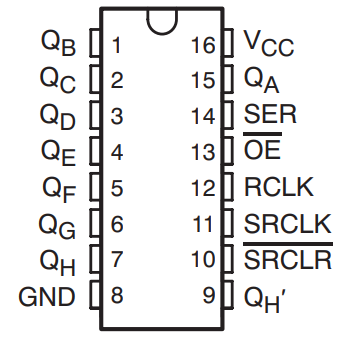
\includegraphics[scale=1]{esquematico.png}
\centering
\caption{Integrado 74HC595.}
\label{fig:int74HC959}
\end{figure}

\textbf{Configuración de pines.}
\newline
\begin{itemize}
\item Los pines de $Q_B$(pin 1) a $Q_H$(pin 7), añadiendo $Q_A$(pin 15) representan las salidas del integrado.
\item $V_C_C$(pin 16) es la alimentación y GND(pin 8) se conecta a tierra.
\item $Q_H$ (pin 9) se utiliza para conectar otro integrado 74HC595 y generar un efecto de cascada.
\item El pin 14 o SER es el pin donde se envían los datos.
\item $\Bar{OE}$(pin 13) llamado Output Enable, habilita las salidas y se activa con un nivel bajo, por lo cual, para que siempre esté activo se conecta a GND.
\item El RCLK (pin 12) es el reloj del registro de almacenamiento y se utiliza para actualizar los datos a los pines de salida.
\item El SRCLK (pin 11) es el reloj que sincroniza la carga de datos.
\item El $\Bar{SRCLR}$ (pin 11) llamado Shift Register Clear, reestablece el registro de desplazamiento.


\end{itemize}

\subsection{Funcionamiento.}\label{integrado funcionamiento}
El objetivo principal es pasar el número dado de un formato serial a uno parelelo. Para explicar el funcionamiento del integrado tomaremos un número cualquiera de 8 bits, este número se irá guardando bit por bit en cada uno de los cuadros que se pueden ver en la Figura \ref{fig:func1}, también podemos ver en esta misma figura que la entrada de los datos es en serie (uno por uno), y la salida de ellos es en paralelo (8 bits).


\begin{figure}[h]
\includegraphics[scale=0.8]{funcionamiento1.png}
\centering
\caption{Representación del funcionamiento del circuito integrado 74HC595.}
\label{fig:func1}
\end{figure}

Para que la toma de los datos sea exitosa es necesario un reloj que por medio de pulsos, controlará en qué momento ingresa al integrado el bit presente en la entrada. Tomaremos de ejemplo la representación binaria del número 49, la cual es 00110001.

El primer paso para transformar la información que se encuentra en serie a paralelo es realizar el desplazamiento de los bits dentro del integrado iniciando por el bit más significativo (MSB por sus siglas en inglés), en nuestro ejemplo es un cero, que se encuentra presente en la entrada y que en el primer pulso del rejol ingresa a la primera posición del registro de desplazamiento. Figura \ref{fig:MSB}

\begin{figure}[h]
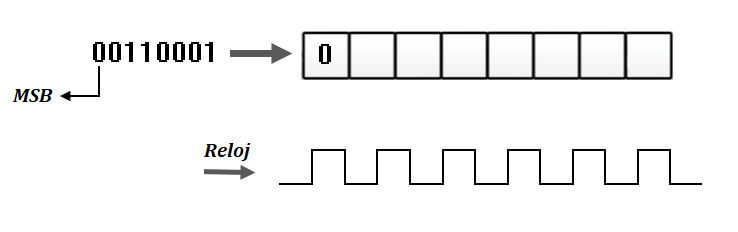
\includegraphics[scale=0.8]{MSB.png}
\centering
\caption{Entrada del MSB al integrado.}
\label{fig:MSB}
\end{figure}

En el próximo pulso del reloj el MSB, ya dentro del integrado, se correrá una posición a la derecha en el registro de desplazamiento, mientras que el número a la derecha del MSB, en la entrada, se posicionará en la primera posición del registro de desplazamiento.

\newpage
\begin{figure}[h]
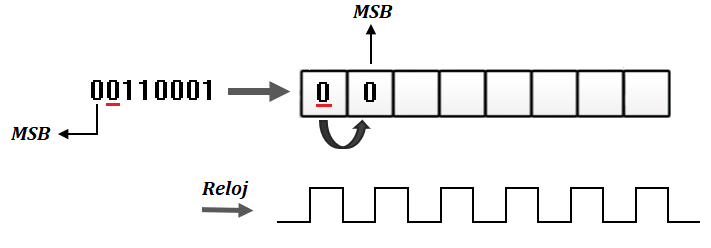
\includegraphics[scale=0.8]{MSB1.png}
\centering
\caption{Desplazamiento de los bits dentro del integrado.}
\label{fig:MSB1}
\end{figure}

Este proceso se repetirá hasta que se ingrese al registro de desplazamiento el último bit del número (Figura \ref{fig:registrolleno}).

\begin{figure}[h]
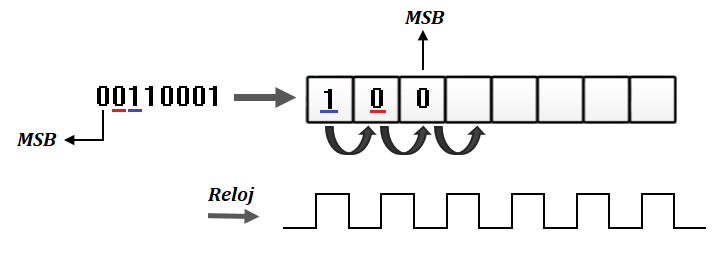
\includegraphics[scale=0.8]{BitsDespla.png}
\centering
\caption{Desplazamiento de los bits dentro del integrado.}
\label{fig:bitsdespla}
\end{figure}

\begin{figure}[h]
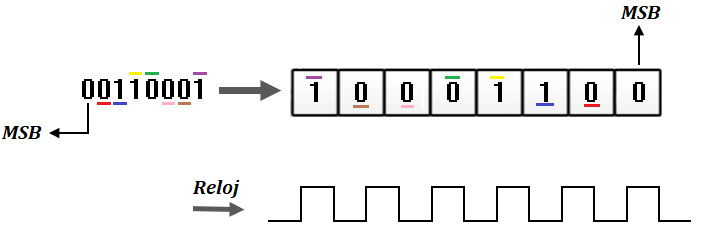
\includegraphics[scale=0.8]{registrolleno.png}
\centering
\caption{Registro de desplazamiento lleno. Se utilizaron colores encima o abajo de los bits para identificar fácilmente cuál es cuál en el registro de desplazamiento.}
\label{fig:registrolleno}
\end{figure}

Para que las salidas no vayan cambiando mientras que el registro de desplazamiento se llena, el integrado hace uso del registro de almacenamiento y el RCLK (Rejol del registro de almacenamiento). Figura \ref{fig:registroalmacenamiento}

\newpage
\begin{figure}[h]
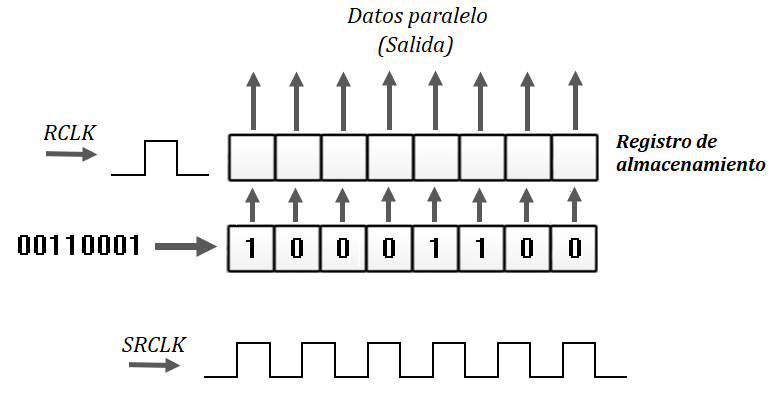
\includegraphics[scale=0.8]{regisalmacen.png}
\centering
\caption{Representación del registro de almacenamiento.}
\label{fig:registroalmacenamiento}
\end{figure}

Una vez se finalice la carga de datos en el registro de desplazamiento, con un único pulso del RCLK se cargan todos los datos del registro de desplazamiento al registro de almacenamiento y se muestran en la salida. De esta forma se alcanzará el objetivo principal, transformar los datos de entrada en serie a datos de salida paralelos.

\begin{figure}[h]
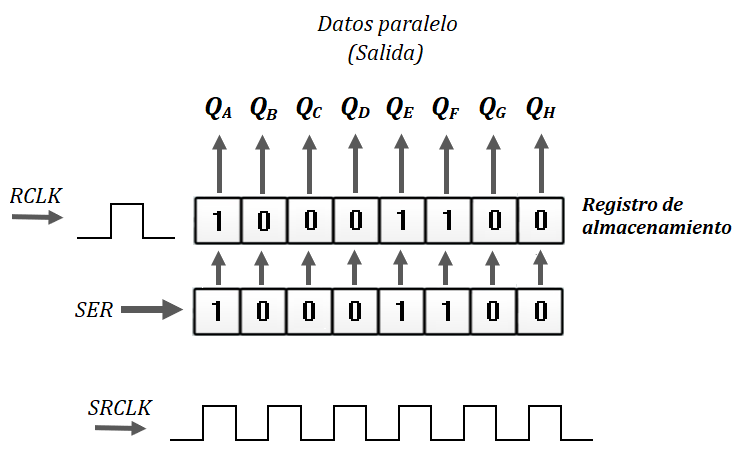
\includegraphics[scale=0.8]{salida.png}
\centering
\caption{Representación del registro de almacenamiento.}
\label{fig:salida}
\end{figure}


\subsection{Aplicaciones.}\label{Aplicaciones}
\begin{itemize}
\item Network switches
\item Power infrastructure
\item LED displays
\item Servers
\end{itemize}

\subsection{Uso del Circuito Integrado 74HC595.}\label{Usocircuito}

\begin{itemize}
\item Con pulsadores: 

\begin{figure}[h]
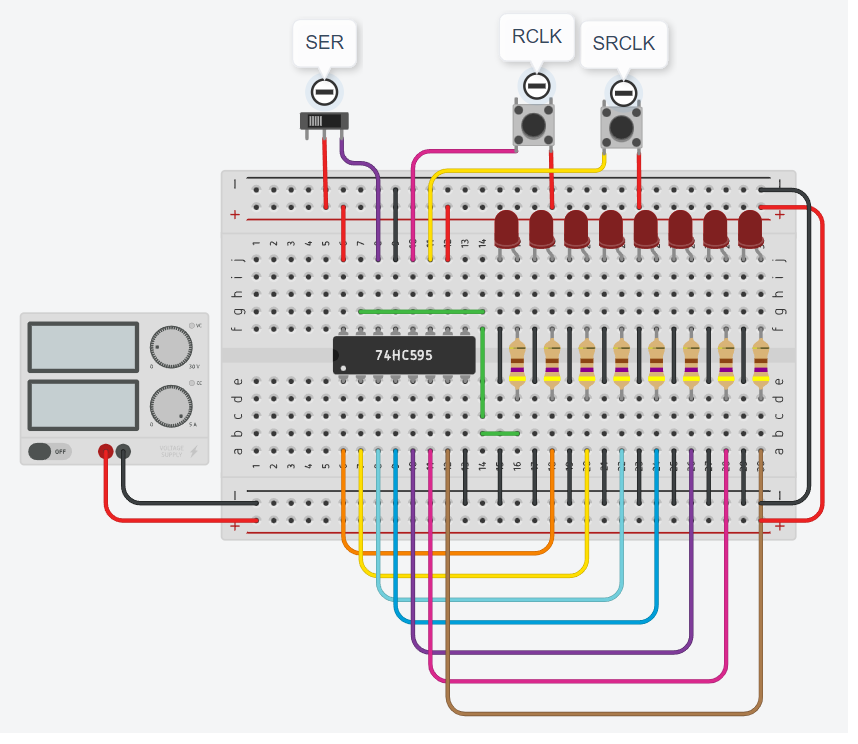
\includegraphics[scale=0.8]{pulsadores.png}
\centering
\caption{Circuito con integrado 74HC595 haciendo uso de pulsadores.}
\label{fig:pulsadores}
\end{figure}

La simulación se puede probar utilizando el siguiente link: https://www.tinkercad.com/things/iBjAIisXge3

\item Con arduino: 

Durante el proceso de implementación fuimos documentando las fases y/o pasos en el desarrolo del integrado con el arduino, de lo cual tenemos la siguiente explicación: \newline
Se define el uso de dos arduinos, montados con su respectiva placa base.
\textbf{Arduino emisor:} \newline
Inicialmente se cuenta con definiciones de macros para este arduino como: TIEMPO, SER, RCLK, SRCLK, TAMAÑO.En variables tenemos la definicion del arreglo donde se utiliza la funcion sizeof, la cual nos permite obtener la longitud de un arreglo, para lo cual toma una variable de entrada de cualquier tipo de datos y devuelve el número de bytes ocupados.

 A continuación se presenta primeramente el montaje del uso del circuito integrado 74HC595 con pulsadores, pero esta vez reemplazando estos últimos con un arduino, para probar así el proceso de emisión del arduino y de recepción del integrado en conjunto.

\begin{figure}[h]
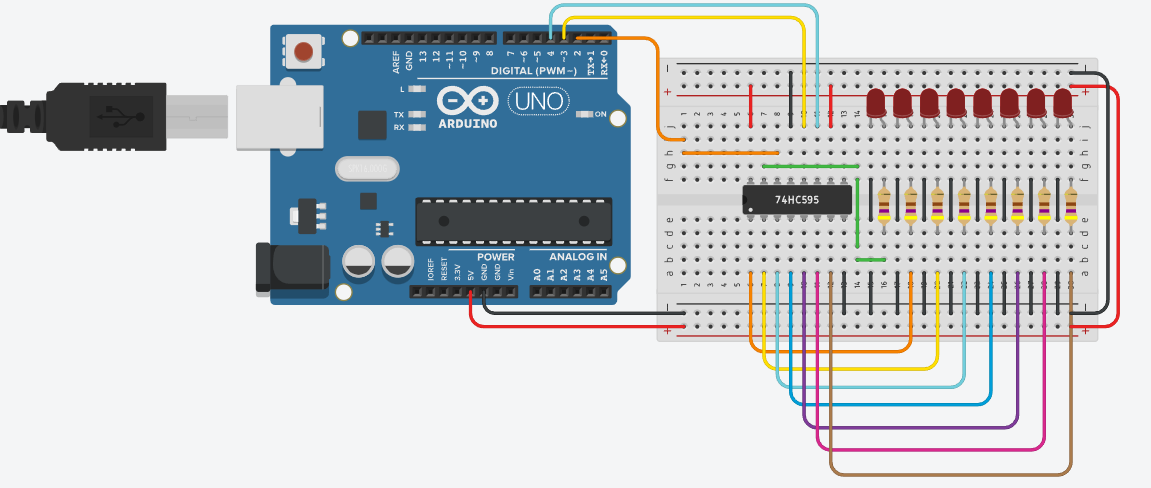
\includegraphics[scale=0.4]{prueba arduino integrado.png}
\centering
\caption{Circuito con integrado 74HC595 haciendo uso de un arduino.}
\label{fig:reemplazo pulsador por arduino}
\end{figure}

\newpage
\begin{lstlisting}[style=myArduino]
//directivas de preprocesamiento
#define tiempo 2000
#define SER 2
#define RCLK 3
#define SRCLK 4


byte codigo[8]={10,255,0,49,50,6,7,8};//A byte stores an 8-bit unsigned number, from 0 to 255.
//----------------------------------------------------------------
//prototipo de las funciones

//----------------------------------------------------------------
//setup
void setup()
{
  for(int i=2;i<5;i++)
  {
    pinMode(i, OUTPUT);
  }
  
}
//----------------------------------------------------------------
//loop
void loop()
{
  for(int i=0;i<8;i++)
  {
  	//delay(25);
    for(int j=0;j<8;j++)
    {
      digitalWrite(SRCLK, LOW);
      digitalWrite(SER, bitRead(codigo[i], j));
      digitalWrite(SRCLK, HIGH);
    }
    //delay(tiempo-25);
    delay(tiempo);
    digitalWrite(RCLK, HIGH);
    digitalWrite(RCLK, LOW);
    
  }
  
  
  
}
//----------------------------------------------------------------
//cuerpo de las funciones
\end{lstlisting}


\end{itemize}


\vspace{0.5cm}
\noindent


\section{Comunicación entre Arduinos} \label{Comunicación entre Arduinos}
\subsection{Intento número 1}\label{intento1}
A continuación se presenta el código y montaje de arduinos que se usaron para probar el tema de comunicación entre dos arduinos. Cabe aclarar que la implementación de estos se dio antes de las indicaciones y especificaciones de la clase del día 17 de febrero, por lo que no reflejan el futuro diseño a implementar, el cual contará con una gran participación del integrado 74HC595 y se sospecha que también del protocolo I2C para la señal de reloj.

\subsubsection{arduino emisor}\label{intento1}

montaje:
\begin{figure}[h]
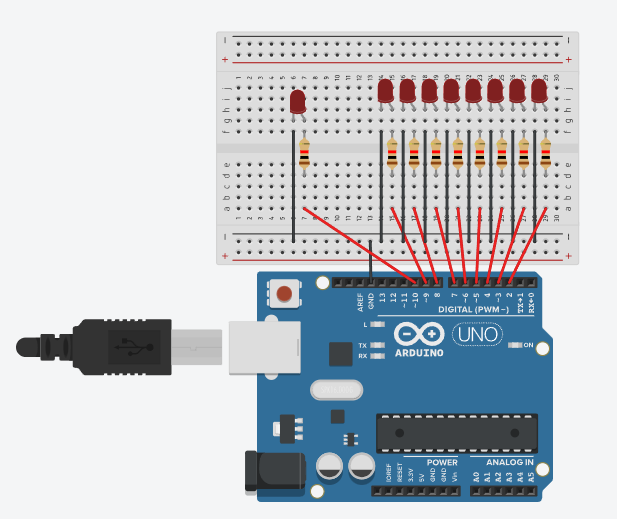
\includegraphics[scale=0.6]{emisor1.png}
\centering
\caption{Prueba de emisión de bits y una señal de reloj por medio de 9 leds.}
\label{fig:emisor1}
\end{figure}

código:
\begin{lstlisting}[style=myArduino]//directivas de preprocesamiento
#define tiempo 1000
byte codigo[8]={1,2,3,4,5,6,7,8};//A byte stores an 8-bit unsigned number, from 0 to 255.
//----------------------------------------------------------------
//prototipo de las funciones

//----------------------------------------------------------------
//setup
void setup()
{
  for(int i=2;i<11;i++)
  {
    pinMode(i, OUTPUT);
  }
  
}
//----------------------------------------------------------------
//loop
void loop()
{
  for(int i=0;i<8;i++)
  {
  	digitalWrite(10, LOW);
  	delay(25); // Wait for 1000 millisecond(s)
    for(int j=0;j<8;j++)
    {
      digitalWrite(j+2, bitRead(codigo[i], j));
    }
    delay(tiempo-25);
    digitalWrite(10, HIGH);
    delay(tiempo);
  }
  
  
}
//----------------------------------------------------------------
//cuerpo de las funciones
\end{lstlisting}


\newpage
\subsubsection{arduino emisor y receptor}\label{intento1}

montaje:
\begin{figure}[h]
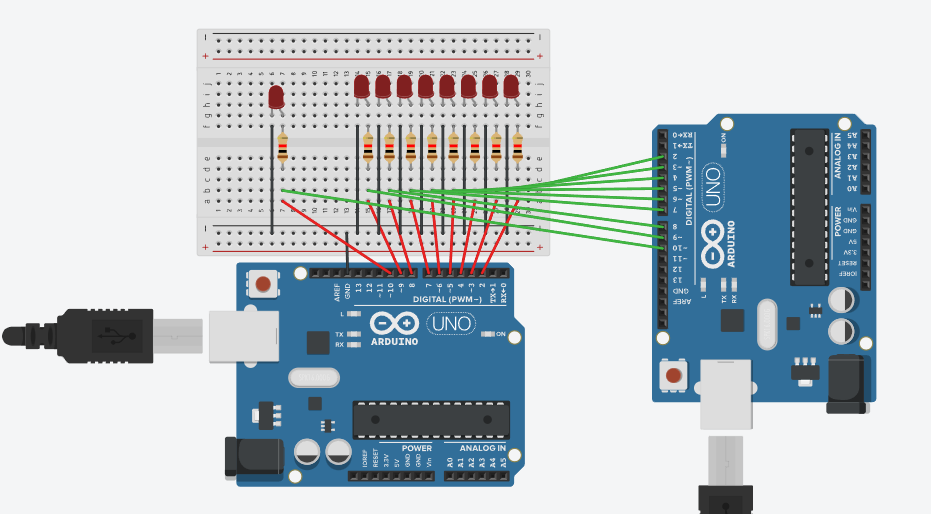
\includegraphics[scale=0.6]{emisorReceptor1.png}
\centering
\caption{Prueba de emisión de bits y una señal de reloj por medio de 9 leds y su recepción a otro arduino.}
\label{fig:emisorReceptor1}
\end{figure}

código arduino emisor:
\begin{lstlisting}[style=myArduino]//directivas de preprocesamiento
//directivas de preprocesamiento
#define tiempo 250
byte codigo[8]={2,1,3,4,5,6,7,8};//A byte stores an 8-bit unsigned number, from 0 to 255.
//----------------------------------------------------------------
//prototipo de las funciones

//----------------------------------------------------------------
//setup
void setup()
{
  for(int i=2;i<11;i++)
  {
    pinMode(i, OUTPUT);
  }
  
}
//----------------------------------------------------------------
//loop
void loop()
{
  for(int i=0;i<9;i++)
  {
  	digitalWrite(10, LOW);
  	delay(50); // Wait for 1000 millisecond(s)
    for(int j=0;j<8;j++)
    {
      digitalWrite(j+2, bitRead(codigo[i], j));
    }
    delay(tiempo-50);
    digitalWrite(10, HIGH);
    delay(tiempo);
  }
  
  
}
//----------------------------------------------------------------
//cuerpo de las funciones
 
\end{lstlisting}

código arduino receptor:
\begin{lstlisting}[style=myArduino]//directivas de preprocesamiento
// C++ code
//
int entero=0;
bool primerCero=false;
void setup()
{
  Serial.begin(9600);
  for(int i=2;i<11;i++)
  {
    pinMode(i, INPUT);
  }
}

void loop()
{
  if(primerCero==true)
  {
    for(int i=0;i<8;i++)
    {
      entero=entero+((int)digitalRead(i+2))*pow(2,i);
    }
    Serial.println(entero);
    entero=0;
    primerCero=false;
  }
  if(primerCero==false)
  {
    while(digitalRead(10)==true)
    {
      primerCero=true;
    }
  }
  
}
 
\end{lstlisting}

\subsection{Intento número 2(protocolo I2C)}\label{intento2}
A continuación se presenta un modelo más cercano a lo que se planea hacer para la comunicación de la señal de reloj y los datos. Para ello usaremos el protocolo I2C.

montaje:
\begin{figure}[h]
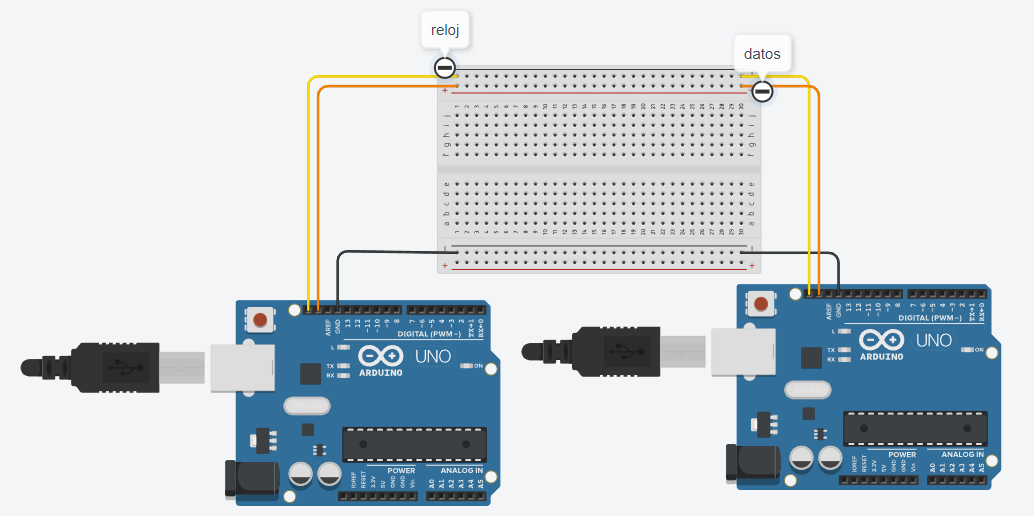
\includegraphics[scale=0.5]{emisorReceptor2.png}
\centering
\caption{Comunicación mediante el protocolo I2C.}
\label{fig:emisorReceptor2}
\end{figure}

Código arduino emisor:
\begin{lstlisting}[style=myArduino]//directivas de preprocesamiento
#include <Wire.h>

// C++ code
//----------------------------------------------------------------
//----------------------------------------------------------------

byte pin[] = {9, 10, 11, 12, 13};
byte estado = 0;
#define retardo 2000
int ValorSensor = 0;

//----------------------------------------------------------------
//----------------------------------------------------------------

void setup()
{
  Wire.begin();
  pinMode(LED_BUILTIN, OUTPUT);
}

//----------------------------------------------------------------
//----------------------------------------------------------------

void loop()
{
  Wire.beginTransmission(1); // Transmite al Esclavo 1
  Wire.write(estado);
  Wire.endTransmission();
  
  digitalWrite(LED_BUILTIN, estado);
  
  delay(retardo);
  
  if (estado == 0)
  {
    estado = 1;
  }
  else
  {
    estado = 0;
  }
}
 
\end{lstlisting}

Código arduino receptor:
\begin{lstlisting}[style=myArduino]//directivas de preprocesamiento
#include <Wire.h>

void llegaDato(int howMany);
// C++ code
//
void setup()
{
  pinMode(13, OUTPUT);    // Pines en modo salida
  Wire.begin(1); // Unimos este dispositivo al bus I2C con dirección 2 (Esclavo 2)
  Wire.onReceive(llegaDato);
  pinMode(LED_BUILTIN, OUTPUT);
}

void loop()
{
  delay(30); // Wait for 1000 millisecond(s)
}

void llegaDato(int howMany){  
  int estado = 0;
  if (Wire.available() == 1) // Si hay un byte disponible
  {
    estado = Wire.read();
  }
  digitalWrite(13,estado);   // Activamos/desactivamos salida depende del Maestro
}
 
\end{lstlisting}

\subsection{Intento número 3: Prueba de conexión entre arduinos usando puertos digitales}\label{intento3}
Tras la sesión de clase del día 25 de febrero, el profesor nos indicó que no había necesidad de recurrir a protocolos como el I2C, por lo que se procedió a hacer una implementación mediante el uso de puertos digitales únicamente. \newline A continuación se presenta primeramente el montaje del uso del circuito integrado 74HC595, para probar así el proceso de emisión del arduino generador , y el proceso de recepción del segundo arduino, a la vez que verificamos con el integrado.
\newline Montaje: \newline \newline \newline

\begin{figure}[h]
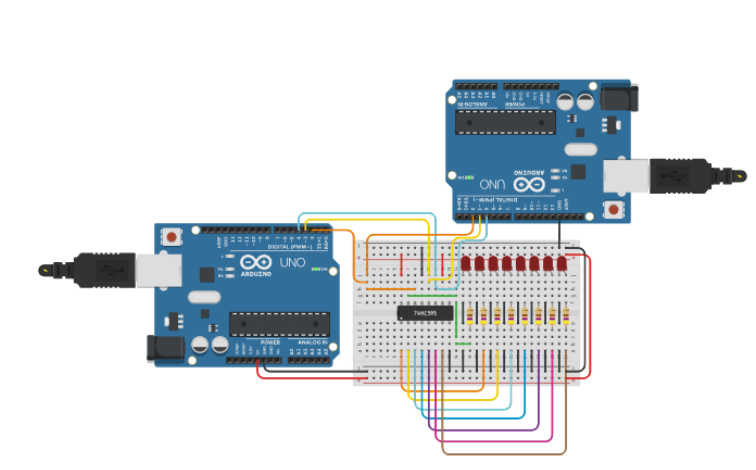
\includegraphics[scale=0.6]{prueba conexión entre arduinos (fallo).png}
\centering
\caption{Comunicación entre arduinos, verificando con la ayuda de 8 leds y el integrado.}
\label{fig:reemplazo pulsador por arduino}
\end{figure}
Lastimosamente, no se pudo codificar de forma correcta, por lo que el proceso de recepción falló.
\newline Código emisor:
\begin{lstlisting}[style=myArduino]
//directivas de preprocesamiento
#define tiempo 2000
#define SER 2
#define RCLK 3
#define SRCLK 4


byte codigo[8]={10,255,0,49,50,6,7,8};//A byte stores an 8-bit unsigned number, from 0 to 255.
//----------------------------------------------------------------
//prototipo de las funciones

//----------------------------------------------------------------
//setup
void setup()
{
  for(int i=2;i<5;i++)
  {
    pinMode(i, OUTPUT);
  }
  
}
//----------------------------------------------------------------
//loop
void loop()
{
  for(int i=0;i<8;i++)
  {
  	//delay(25);
    for(int j=0;j<8;j++)
    {
      digitalWrite(SRCLK, LOW);
      digitalWrite(SER, bitRead(codigo[i], j));
      digitalWrite(SRCLK, HIGH);
    }
    //delay(tiempo-25);
    delay(tiempo);
    digitalWrite(RCLK, HIGH);
    digitalWrite(RCLK, LOW);
    
  }
  
  
  
}
//----------------------------------------------------------------
//cuerpo de las funciones
\end{lstlisting}

Código receptor:
\begin{lstlisting}[style=myArduino]
#define SER 2
#define RCLK 3
#define SRCLK 4

void setup()
{
  Serial.begin(9600);
  for(int i=2;i<5;i++)
  {
    pinMode(i, INPUT);
  }

}

void loop()
{
  if(digitalRead(RCLK))
  {
    if(digitalRead(SRCLK))
    {
      for(int i=0;i<8;i++)
      {
        Serial.print(digitalRead(2));
      }
      Serial.println();
    }
  }
}
\end{lstlisting}

\subsection{Intento número 4 (conexión entre arduinos (funciona:muestra bin y dec))}\label{intento4}
Tras varias horas de prueba se consigue una comunicación exitosa entre ambos arduinos, no solo mostrando los números en formato binario, sino también en décimal. (el montaje es el mismo del intento número 3).

Código:
\begin{lstlisting}[style=myArduino]
//directivas de preprocesamiento
#define tiempo 1000
#define SER 2
#define RCLK 3
#define SRCLK 4


byte codigo[8]={1,2,255,0,50,6,7,8};//A byte stores an 8-bit unsigned number, from 0 to 255.
int tamanoArray=sizeof(codigo)/sizeof(byte);
//----------------------------------------------------------------
//prototipo de las funciones

//----------------------------------------------------------------
//setup
void setup()
{
  for(int i=2;i<5;i++)
  {
    pinMode(i, OUTPUT);
    digitalWrite(i, LOW);
  }
}
//----------------------------------------------------------------
//loop
void loop()
{
  for(int i=0;i<tamanoArray;i++)
  {
    for(int j=0;j<8;j++)
    {
      digitalWrite(SER, bitRead(codigo[i], j));
      digitalWrite(SRCLK, HIGH);
      delay(100);
      digitalWrite(SRCLK, LOW);

    }
    delay(tiempo);
    digitalWrite(RCLK, HIGH);
    digitalWrite(RCLK, LOW);
    
  }
  
  
  
}
//----------------------------------------------------------------
//cuerpo de las funciones
\end{lstlisting}

Código:
\begin{lstlisting}[style=myArduino]
#define SER 2
#define RCLK 3
#define SRCLK 4

bool leerBit=true;
byte binario[8];

byte bintodec(byte* bin);
byte dos_exp (int exp);

void setup()
{
  Serial.begin(9600);
  for(int i=2;i<5;i++)
  {
    pinMode(i, INPUT);
  }
}

void loop()
{
  
  if(digitalRead(SRCLK))
  {
    for(int i=0;i<8;i++)
    {
      while(!digitalRead(SRCLK))
      {
        
      }
      binario[i]=digitalRead(SER);
      while(digitalRead(SRCLK))
      {
        
      }
    }
    delay(1000);
    for(int i=7;i>=0;i--)
    {
      Serial.print(binario[i]);
    }
    Serial.println();
    Serial.println(bintodec(binario));
  }
}
//--------------------------------------------------------------
//funciones
byte bintodec(byte * bin){ // recibe un binario y retorna un decimal en tipo entero
    byte dec = 0;
    for(int i=7; i>=0 ; i--){
        if (bin[i]>=1){
                dec = dec + (dos_exp(i));
        }
    }
    return dec;
}

byte dos_exp (int exp){
    int acu = 1;
    for (int i=0 ; i<exp ; i++){
        acu = acu*2;
    }
    return acu;
}
\end{lstlisting}

\subsection{Intento número 4 mejorado (implementacion lcd bin y dec)}\label{intento4}
Una vez funciona la comunicación entre arduinos, se procede a traspasar el codigo, de modo que el despliegue de información pase del monitor serial, como venía mostrándose, a un display lcd.

Montaje:

\begin{figure}[h]
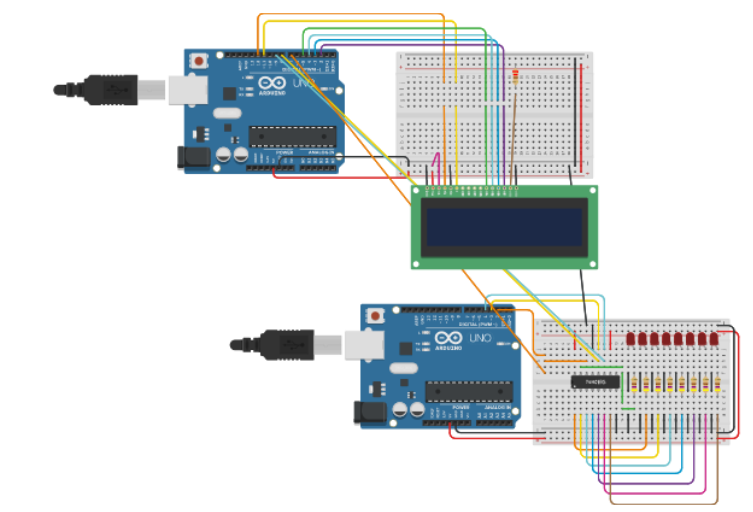
\includegraphics[scale=0.6]{implementacion lcd bin y dec.png}
\centering
\caption{Conexión arduinos con lcd.}
\label{fig:reemplazo pulsador por arduino}
\end{figure}

Código emisor:
\begin{lstlisting}[style=myArduino]
//directivas de preprocesamiento
#define tiempo 1000
#define SER 2
#define RCLK 3
#define SRCLK 4


byte codigo[8]={1,2,255,0,50,6,7,8};//A byte stores an 8-bit unsigned number, from 0 to 255.
int tamanoArray=sizeof(codigo)/sizeof(byte);
//----------------------------------------------------------------
//prototipo de las funciones

//----------------------------------------------------------------
//setup
void setup()
{
  for(int i=2;i<5;i++)
  {
    pinMode(i, OUTPUT);
    digitalWrite(i, LOW);
  }
}
//----------------------------------------------------------------
//loop
void loop()
{
  for(int i=0;i<tamanoArray;i++)
  {
    for(int j=0;j<8;j++)
    {
      digitalWrite(SER, bitRead(codigo[i], j));
      digitalWrite(SRCLK, HIGH);
      delay(100);
      digitalWrite(SRCLK, LOW);

    }
    delay(tiempo);
    digitalWrite(RCLK, HIGH);
    digitalWrite(RCLK, LOW);
    
  }
  
  
  
}
//----------------------------------------------------------------
//cuerpo de las funciones
\end{lstlisting}

Código receptor:
\begin{lstlisting}[style=myArduino]
// include the library code:
#include <LiquidCrystal.h>

// initialize the library with the numbers of the interface pins
LiquidCrystal lcd(12, 11, 5, 4, 3, 2);

#define SER 7
#define RCLK 8
#define SRCLK 9

byte bintodec(byte * bin);
byte binario[8];

byte dos_exp (int exp);

void setup() {
  // set up the LCD's number of columns and rows:
  lcd.begin(16, 2);
  
  for(int i=7;i<10;i++)
  {
    pinMode(i, INPUT);
  }
}

void loop() {
  
  if(digitalRead(SRCLK))
  {
    for(int i=0;i<8;i++)
    {
      while(!digitalRead(SRCLK))
      {
        
      }
      //Serial.print(digitalRead(2));
      binario[i]=digitalRead(SER);
      while(digitalRead(SRCLK))
      {
        
      }
    }
    delay(1000);
    lcd.clear();
    for(int i=7;i>=0;i--)
    {
      lcd.print(binario[i]);
    }
    lcd.setCursor(0, 1);
    lcd.print(bintodec(binario));


  }
  // print the number of seconds since reset:
  //lcd.print(millis() / 1000);
}


//funciones
byte bintodec(byte * bin){ // recibe un binario y retorna un decimal en tipo entero
    byte dec = 0;
    for(int i=7; i>=0 ; i--){
        if (bin[i]>=1){
                dec = dec + (dos_exp(i));
        }
    }
    return dec;
}

byte dos_exp (int exp){
    int acu = 1;
    for (int i=0 ; i<exp ; i++){
        acu = acu*2;
    }
    return acu;
}
\end{lstlisting}


\section{Cibergrafía} \label{ciber}

https://www.electrogeekshop.com/como-funciona-el-74hc595-shift-register-y-su-interfaz-con-arduino/
\newline
https://github.com/trihedral/ArduinoLatexListing
\newline
https://www.youtube.com/watch?v=9gfZnNPBlVg

\end{document}
